\chapter{Background}\label{background}

    This chapter aim to explain technologies, tools, and specification of a device that are used in this project.
    Then, this chapter gives an analysis of related applications.

    \section{Android Application}
        -	What is Android
            - An open source OS, support mobiles, tablets, watches, TVs, Cars’ system [http://tinyurl.com/yag8kyst]
        -	Android development
            - IDE -> Android studio which provides SDKs and tools
            - Native application -> Java and Kolin
            - Native language -> C and C++
                1.	For intensive application which require extra performance
                2.	Accessing native libs (C and C++)
            - Java and C++ communicate by using Java Native Interface (JNI) [https://developer.android.com/ndk/guides]
                - What is JNI
                - Why I need this

        % -	Server (and Cloud) is replaced by Mobile Computing [http://tinyurl.com/y6vusamh]
        % -	Mobile edge cloud [http://tinyurl.com/y7umteqg]

    \section{Human Detection}
        -	People Detection
            - Using DNN
            - What is DNN
            - How it works
            - How it works in this project
                - Insert diagram of DNN (Flow of Image Processing)
                    - blobFronImage
                    - forward
                    - ...

    \section{Distance Calculation}
        To measure a distance between 2 people, the reference point of people are used for calculation.
        The reference point is the coordination of each people, which is the centre of the detection frame.
        The calculation formula is based on Euclidean distance.

        \begin{equation*}
            d = \sqrt{(a_{0}-b_{0})^{2}+(D/c)\times(a_{1}-b_{1})^{2}}
        \end{equation*}

        \begin{equation*}
            c = \frac{a_{1}+b_{1}}{2}
        \end{equation*}

        However, three-dimensional space are captured into two-dimensional image, so depth and perspective are concerned.
        Thus, a couple variables are added into the formula.
        The first variable is $D$, which is the diagonal of the image.
        The second variable is $c$, which is a calibration.
        These 2 variables will determine the depth of people in the image.

        \begin{figure}[!ht]
            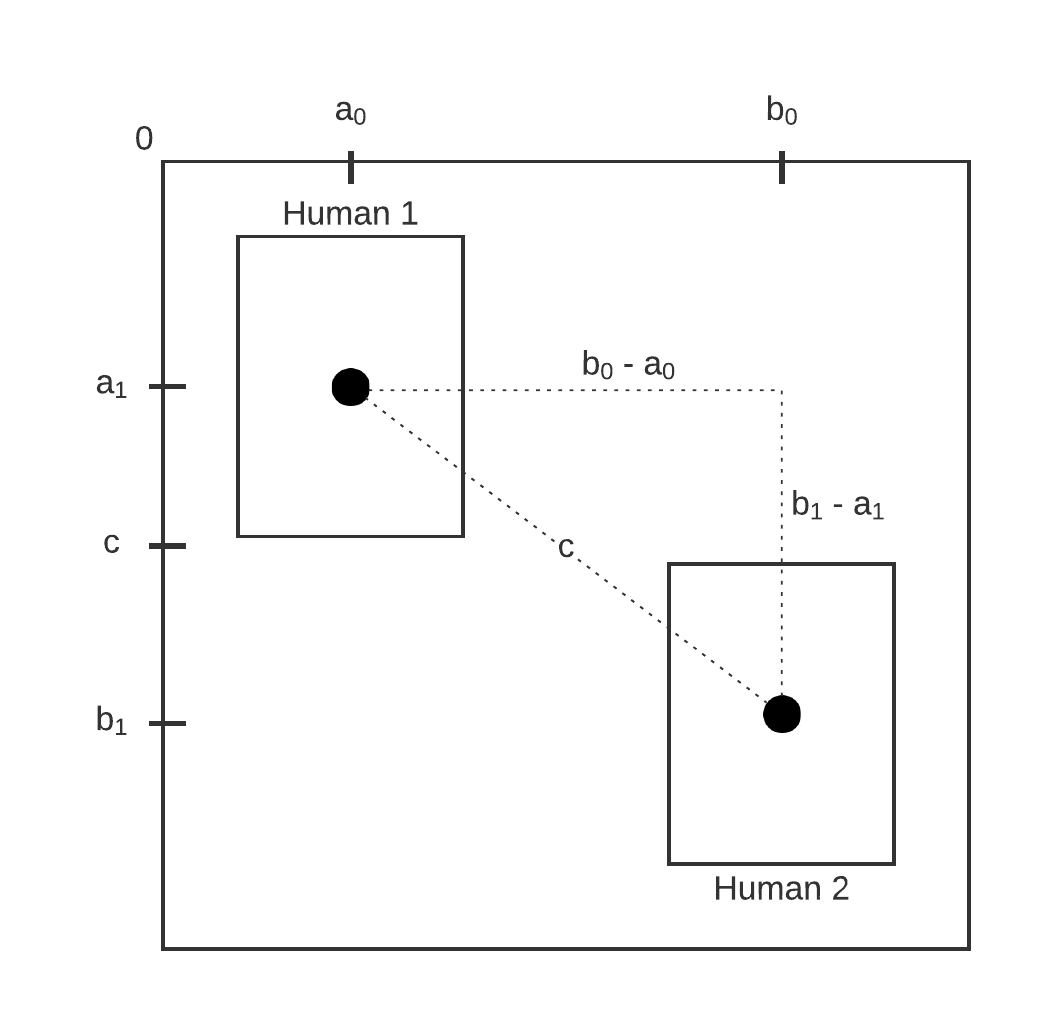
\includegraphics[width=6in]{images/chapter2/distance.png}
            \caption{Distance Calculation}
            \label{distanceCalculation}
        \end{figure}

        For example, according to the figure \ref{twoDistances},
        if distance is calculated without calibration, distance between 2 couples will be the same.
        Naturally, the distance between Human1 and Human2 must be further than the distance between Human3 and Human4.

        \begin{figure}[!ht]
            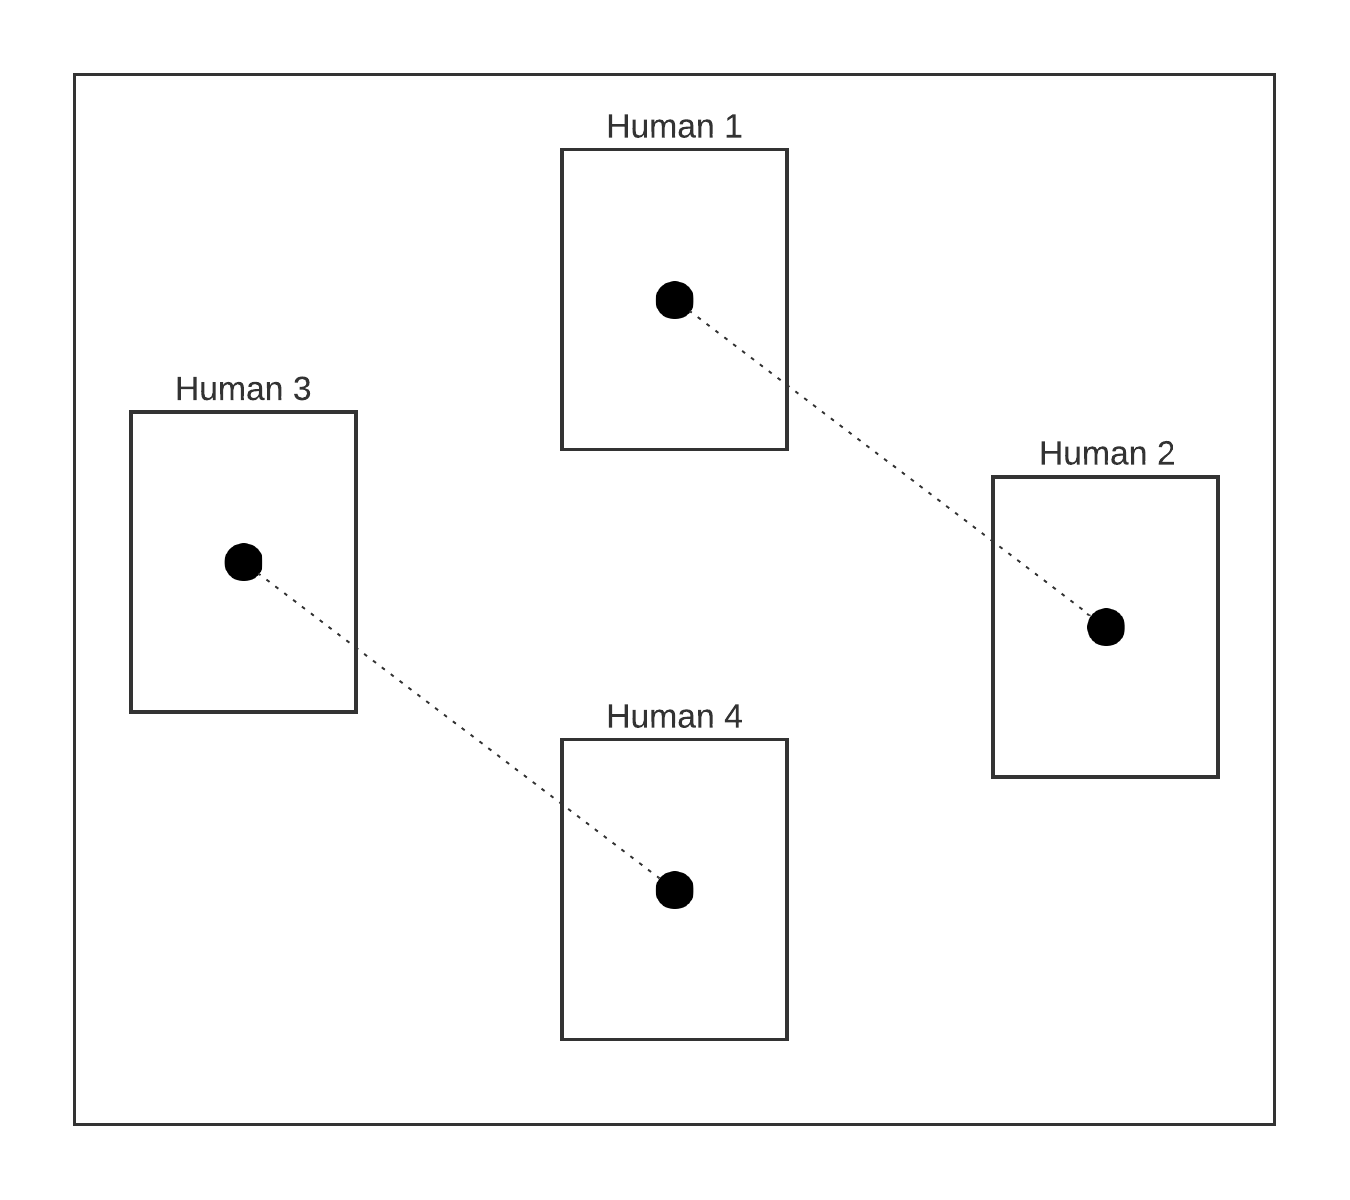
\includegraphics[width=6in]{images/chapter2/two-distances.png}
            \caption{Distance Comparison}
            \label{twoDistances}
        \end{figure}

    \section{Parallel Computing}
        -	What is parallel computing \\
        -   Multithreading \\
        -	Why I need it \\
        -	How it works \\
            - new Thread() vs ThreadPool \\
            - Insert general picture about Parallel computing\\
        -	Why it benefits for Android\\


    \section{Specification}
        This application is developed and tested on following specification:

        \begin{table}[!htp]\centering
            \caption{Specification}\label{tab: }
            \scriptsize
            \begin{tabular}{lrll}\toprule
                Device              &Device             &Samsung S10+ \\ \hline
                Operating System    &Operating System   &Android 10 (Q) \\ \hline
                Processor           &CPU                &Samsung Exynos 9820 \\
                                    &Cores              &8 \\
                                    &Architecture       &2x ARM Cortex-A75 2.73GHz \\
                                    &                   &4x ARM Cortex-A55 1.95GHz \\
                                    &                   &2x Samsung Exynos M4 1.95 GHz \\
                                    &GPU                &Mali-G76 \\ \hline
                Memory              &RAM                &8 GB \\
                \bottomrule
            \end{tabular}
        \end{table}


    \section{Existing Applications}
        1.	Object Detector
            -	250-300 ms per frame
            -	Live camera
        2.	Computer Vision Detection
            -	Don’t know about (ms per frame) or (frame per second)
            -	Live camera – not smooth
            -	Lots of features including face detection
            -	Problem is it still delay
